% Chapter 1

\chapter{Vórtices} % Chapter title

\label{ch:introduction} % For referencing the chapter elsewhere, use \autoref{ch:introduction} 

%----------------------------------------------------------------------------------------

Los vórtices son solitones\footnote{Solitones son soluciones estáticas de las ecuaciones de movimiento (no lineales) de una teoría que son estables, localizados en el espacio y tienen energía finita[solibranas].} en dos dimensiones con comportamiento de partícula que aparecen en ciertas teorías de campo.
Teorías de campo que presentan soluciones vorticiales pueden ser de dos tipos, globales y con gauge, y sus respectivas soluciones son llamadas vórtices globales y vórtices gauge. En una teoría global el único campo dinámico es un campo escalar complejo $\phi(x)$, mientras que en un teoría con gauge este campo se encuentra acoplado al campo electromagnético mediante un potencial de gauge $A_\mu(x)$. 

En este trabajo estamos interesados en el modelo abeliano de Higgs, que es la versión relativista del modelo de Ginzburg-Landau para la superconductividad, la cuál presenta soluciones vorticiales. Empezaremos explicando el modelo de Ginzburg-Landau para la superconductividad.

\section{Modelo de Ginzburg-Landau}

Uno de primeros modelos que explicaron la superconductividad apareció en los años cincuenta de la mano de V. Ginzburg y L. Landau.  Siguiendo el modelo de transiciones de fase de la termodinámica, el "grado de superconductividad" de un cuerpo que ocupa una región del espacio $\om\in\m R^3$, está caracterizado por un parámetro de orden representado como una "pseudo función de onda" $\phi:\om\ra\m C$. En la terminología moderna, $\phi$ es una sección en un fibrado lineal $\hat{\mc L}$.

\subsection{Funcional de energía}

El funcional de energía para un superconductor propuesta por Ginzburg y Landau se puede escribir como
\begin{align}
  V = \f 12\int_\om\bp{|d_A \phi|+\f{\lambda}4(m^2-|\phi|^2)^2}d^3x \label{eq:1} 
\end{align}
Este funcional tiene sus mínimos cuando $|\phi|=m$ y $d_A\phi=0$, asumiendo que $\lambda>0$. Donde $d_A=d-ieA$ es la extensión covariante de la derivada exterior.

\subsection{El efecto Meissner}

El hecho de que $\phi\neq 0$ con $d_A\phi=0$ implica que la curvatura de $\hat{\mc L}$ es cero dentro del material superconductor. Explícitamente, $d_A\phi=0$ implica que $0=d_A^2\phi=-2ieF\phi$, de modo que $F=0$ siempre y cuando $\phi$ sea no nula. Este fenómeno es lo que se conoce como el efecto Meissner: el campo magnético se anula muy dentro del superconductor. Si una esfera de plomo es colocada en el seno de un campo magnético constante, entonces a altas temperaturas el campo magnético no es afectado por la esfera, sin embargo, debajo de una temperatura crítica (usualmente debajo de los 7.2 Kelvin) la esfera se vuelve superconductora y el campo magnético es expedido del interior, como se muestra en la siguiente figura

\begin{figure}[ht]
	\centering
	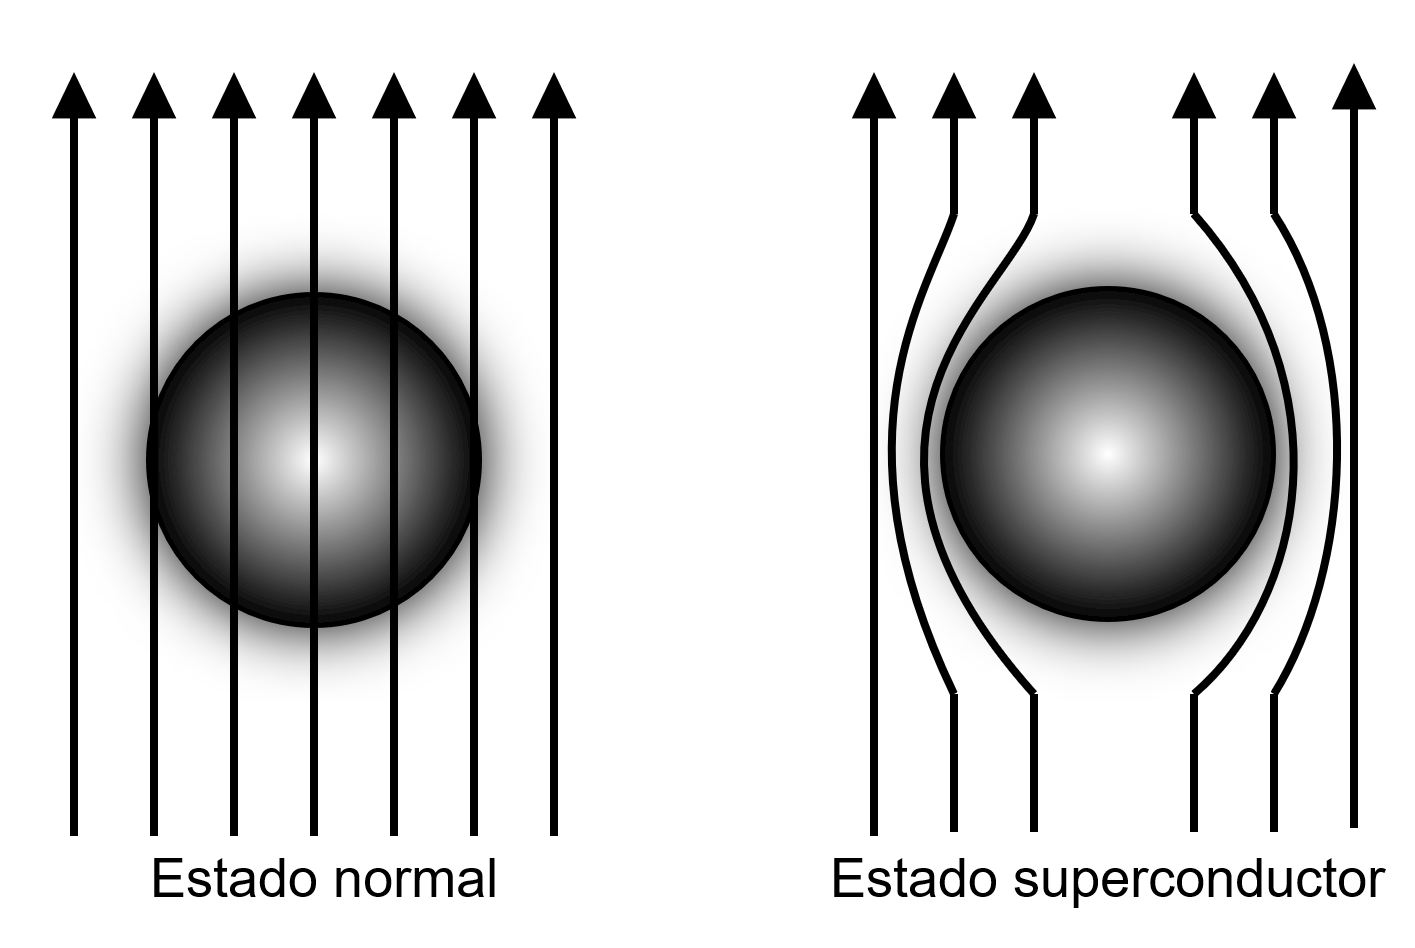
\includegraphics[width=0.6\textwidth]{gfx/superconductingsphere.png}
	\caption{Esfera de plomo en el seno de un campo magnético. A la izquierda por encima de la temperatura crítica. A la derecha el campo magnético es expulsado del interior de la esfera.}
	\label{fig:1}
\end{figure}

Esta explicación del esfecto Meissner recae en la suposición de que el campo magnético no es muy fuerte. Sea $\mc V$ el volumen de la esfera de plomo en fig. \ref{fig:1}. Si hacemos $\phi=0$ en toda la esfera, entonces el campo magnético puede penetrar libremente y de acuerdo a la ecuación \eqref{eq:1}, la energía es $\lambda m^4\mc V/8$. Si hacemos $\phi=m$, el campo es expedido del material y de acuerdo al funcional de energía, esto tiene un costo energético de aproximadamente $|B|^2\mc V/2$. El efecto Meissner ocurrirá si es favorecido energéticamente, esto pasa cuando la energía para expedir el campo magnético es menor a la energía para hacer $\phi=0$. Esto pasa cuando $B$ es menor a un valor crítico $B_{c}=\lambda^{1/2}m^2/2$. Este valor crítico es típicamente del orden de 10000 veces el campo magnético de la Tierra y está cerca de los imanes más potentes actualmente.

Ya que la energía para expedir al campo magnético es proporcional a $|B|^2$, la energía crece cuando $B$ aumenta. Como resultado de esto, un superconductor es repelido de una región donde el campo magnético es grande. Esto lleva al fenómeno de la levitación magnética (fig. \ref{fig:2}).

\begin{figure}[ht]
	\centering
	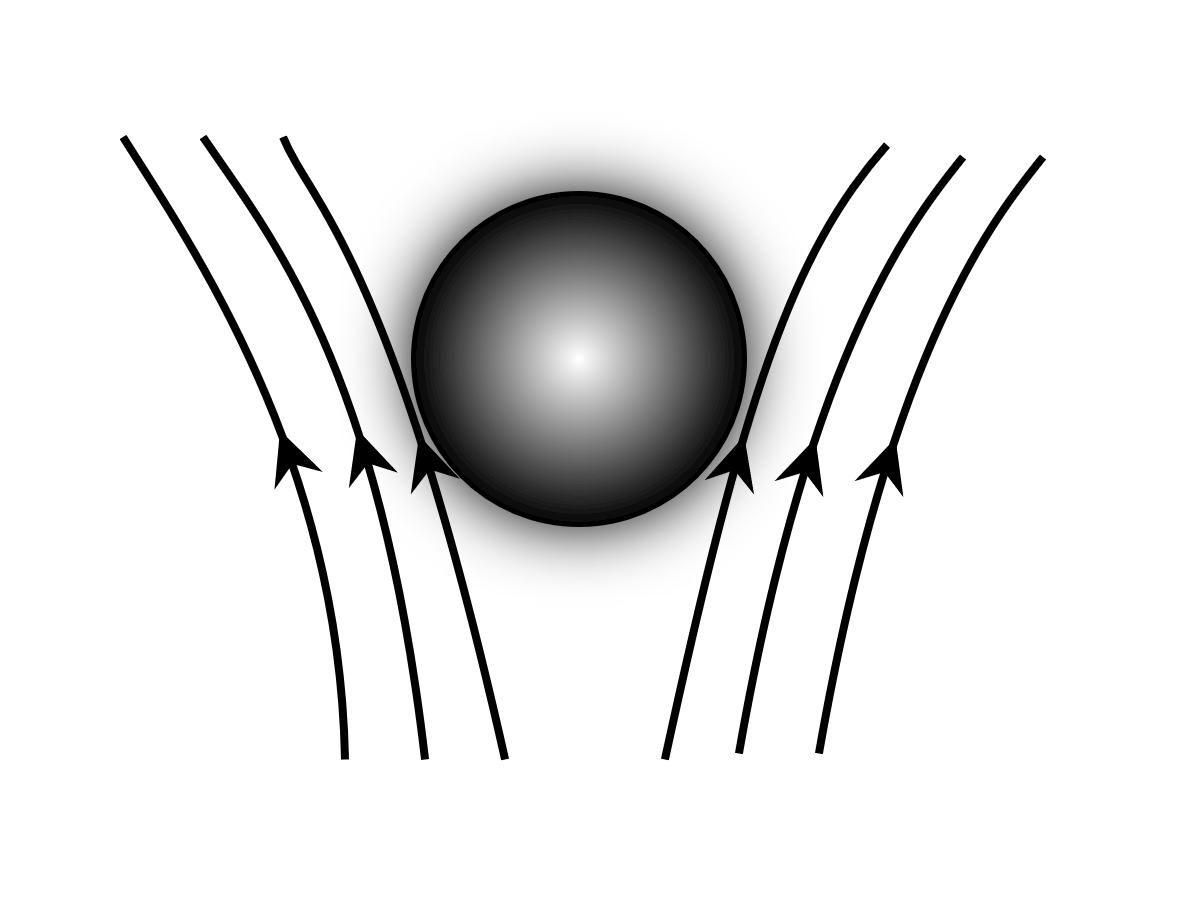
\includegraphics[width=0.6\textwidth]{gfx/maglev.png}
	\caption{Esfera superconductora es repelida de una región donde el campo magnético es fuerte.}
	\label{fig:2}
\end{figure}

Un material superconductor presenta corrientes eléctricas que fluyen en su interior y que son los responsables de cambiar la configuración del campo externo mostrado en fig. \ref{fig:2}. Las corrientes dentro del superconductor crean un campo magnético tal que la suma del campo externo con este campo interno se anula. Estas corrientes fluyen indefinidamente, ya que el efecto Meissner es energéticamente favorable. El hecho de que estas corrientes fluyan indefinidamente sin gasto energético es lo que conocemos como superconductividad.

Las ecuaciones de Maxwell independientes del tiempo demandan de que si el campo magnético es nulo en el interior de un superconductor, entonces la densidad de corrientes $\vec J$ también. Por lo tanto, las corrientes deben fluir en la superficie del material.

\subsection{Líneas de flujo}

Una línea de flujo es una región unidimensional dentro del superconductor donde la sección $\phi=0$. Estas líneas de flujo son de gran importancia científica y tecnológica y son conocidas como líneas de flujo de Abrikosov-Gorkov. Una representación de estas líneas de flujo en una esfera superconductora se muestra en figura \ref{fig:3}

\begin{figure}[ht]
	\centering
	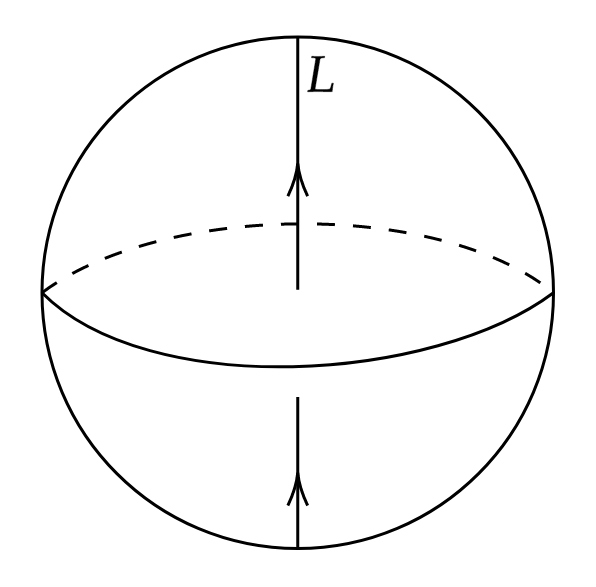
\includegraphics[width=0.5\textwidth]{gfx/fluxline.png}
	\caption{Linea de flujo dentro de una esfera superconductora. A lo largo de la línea $\phi=0$.}
	\label{fig:3}
\end{figure}

Podemos describir matemáticamente a las líneas de flujo como mínimos de un funcional de energía adecuado. En el modelo de Ginzburg-Landau, la función de energía es la suma de la energía para $\phi$, dada en \eqref{eq:1}, y la energía magnética, que es la integral de $|B|^2/2$. La función a minimizar es
\begin{align}
	V(\phi,B) = \int_{\m R^3}d^3x\bp{\f{|B|^2}2+\f 12|d_A\phi|^2+\f{\lambda}{8}(m^2-\phi^2)^2}.
\end{align}
Las ecuaciones de Euler-Lagrange nos devuelven las ecuaciones de la teoría de Ginzburg-Landau:
\begin{align}
	D_\mu D^\mu\phi+\f{\lambda}4\phi(m^2-\phi^2) &=0\\
	\eps_{ij}B_i+ie(\bar\phi D_j\phi-\phi\bar{D_i\phi}) &=0
\end{align}
Estas ecuaciones en derivadas parciales se pueden reducir a ecuaciones diferenciales ordinarias usando argumentos de simetría (como veremos en la sección \ref{sec:1.3}) en $\m R^2$. Soluciones a estas ecuaciones con el típico comportamiento $|\phi|\ra m$ y $d_A\phi\ra 0$ en el infinito son caracterizadas por un entero $n$, conocido como la primera clase de Chern. Soluciones existen, pero no se pueden escribir en una forma explícita, incluso la solución más básica de la línea vorticial de Abrikosov-Gorkov con $n=1$.

\subsection{Superconductores Tipo I y Tipo II}

Podemos reescalear la energía de Ginzburg-Landau de modo que sólo dependa de una constante adimensional. Considere los siguientes reescaleos: la sección $\phi$ puede ser reescaleada como $\phi\ra\phi/a$, las nuevas coordenadas espaciales $x\ra emx$, la conexión $A\ra eA$ y la curvatura $F\ra eF$. Con estas definiciones la constante de acoplamiento se vuelve adimensional $\lambda\ra\lambda/e^2$.

Una transición de fase ocurre cuando $\lambda=1$. Considere una superconductor que llena todo el espacio $\m R^3$ que posee líneas de flujo. Para $\lambda<1$, las líneas de flujo se atraen y se combinan para formar una sólo línea de flujo. Estos materiales son llamadas superconductores tipo I; ejemplos incluyen muchos metales puros. Para $\lambda>1$, las líneas de flujo se repelen. Un material con esta propiedad es llamado un superconductor tipo II.

La distinción de estos dos tipos de superconductores es de gran importancia práctica. Cuando un campo magnético externo se comienza a acercar al campo magnético crítico, líneas de flujo comienzan a penetrar el material. En superconductores Tipo I, estas líneas se atraen, provocando una región no superconductora (líneas de flujo la atraviesan) que va creciendo conforme seguimos aumentando el campo; eventualmente, la superconductividad se pierde. En el caso de superconductores Tipo II, las líneas de flujo se repelen, pudiendo formar un arreglo estable (fig. \ref{fig:4}). Como resultado, un superconductor Tipo II puede mantener su superconductividad incluso para campos magnéticos por encima del valor crítico, haciéndolos más útiles para aplicaciones tecnológicas.  Aún así, llegado a un segundo valor crítico del campo magnético, la superconductividad se pierde.

\begin{figure}[ht]
	\centering
	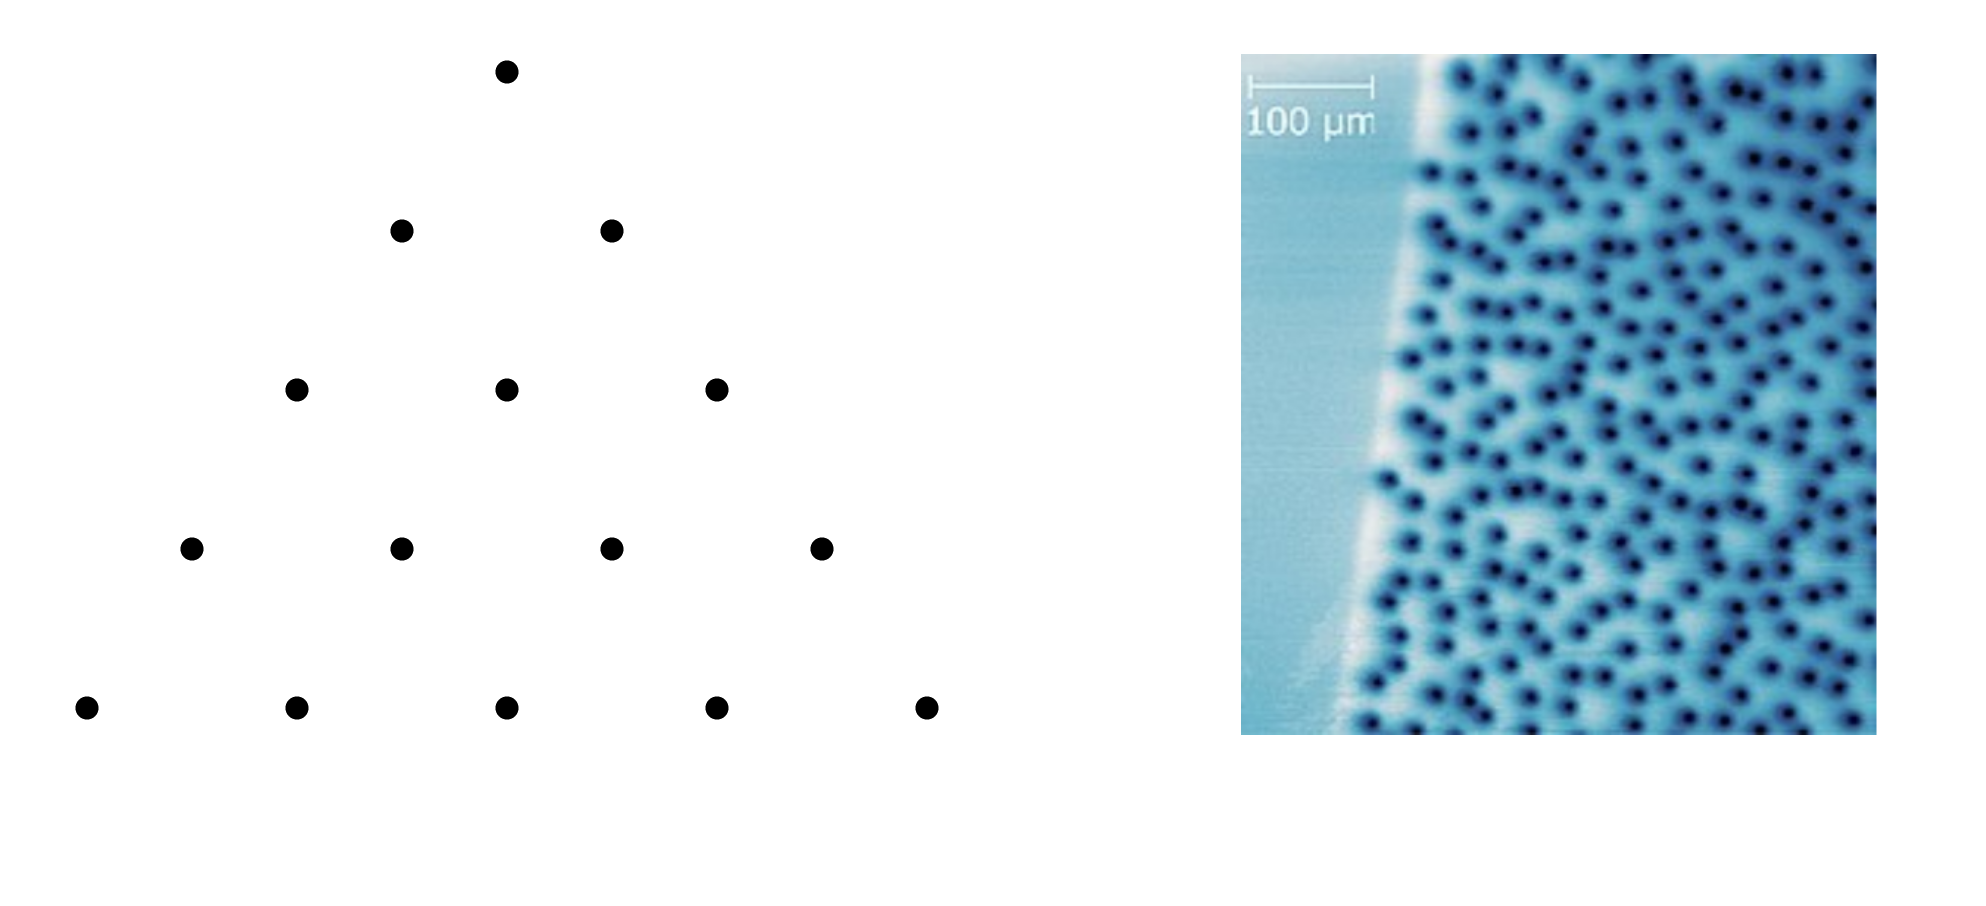
\includegraphics[width=0.6\textwidth]{gfx/type2superconductor.png}
	\caption{A la izquierda, un arreglo estable de líneas de flujo vistas desde arriba. A la derecha vórtices en una lámina delgada de 200 nm de YBCO, tomada usando microscopía SQUID.}
	\label{fig:4}
\end{figure}


\section{Modelo de Higgs abeliano}

El modelo de Higgs abeliano (o modelo de Maxwell-Higgs) es la versión relativista del modelo GL. La sección $\phi(x):\m R^{2+1}\ra\m C$ se le conoce ahora como campo de Higgs. Esta teoría es el paradigma para obtener soluciones vorticiales. La densidad lagrangiana de la teoría es
\begin{align}
    \mc L = -\f 14 F_{\mu\nu}F^{\mu\nu}+\f 12D_\mu\phi\overline{D^\mu\phi}-\f{\lambda}8(1-|\phi|^2)^2 \label{eq:2}
\end{align}
Este funcional corresponde a una teoría gauge pues el campo de Higgs se encuentra acoplado al campo electromagnético. La teoría tiene presenta las simetrías internas típicas del electromagnetismo, i.e., invarianza ante transformaciones de gauge $\phi\ra e^{i\al}\phi$ y $A_\mu\ra A_\mu-i\pr_\mu\al$. Las correspondientes ecuaciones de Euler-Lagrange son
\begin{align}
    D_\mu D^\mu\phi + \f{\lambda}2(1-|\phi|^2)\phi &=0,\label{eq:euler1}\\
    \pr_\mu F^{\mu\nu} &= J^\nu,\label{eq:euler2}
\end{align}
donde $J^\mu=\f i2(\bar\phi D^\mu\phi-\overline{D^\mu\phi}\phi)$ puede ser considerada como una \emph{corriente} generada por la simetría interna. Buscamos configuraciones de campos vorticiales, esto es, soluciones estáticas a $\eqref{eq:euler1}$ y $\eqref{eq:euler2}$ con energía finita. En el gauge temporal $A_0=0$, el funcional de energía de la configuración estática es
\begin{align}
    V_{\lambda} = \f 12\int_{\m R^2}\bp{B^2+D_i\phi\overline{D_i\phi}+\f{\lambda}4(1-|\phi|^2)^2}d^2x \label{eq:gl}
\end{align}
Podemos obtener la correspondiente teoría global haciendo $A_i=0$, obteniéndose
\begin{align}
    V_{\lambda} = \f 12\int_{\m R^2}\bp{|\nabla\phi|^2+\f{\lambda}4(m^2-|\phi|^2)^2}d^2x \label{eq:3a}
\end{align}
A esta teoría global se la conoce como teoría de Ginzburg-Landau global y sus soluciones son llamadas vortices globales. En este trabajo estamos especialmente interesados en el modelo de Higgs abeliano, sin embargo, analizaremos brevemente la teoría de Ginzburg-Landau global ya que algunos métodos nos servirán más tarde.

\section{Teoría de Ginzburg-Landau global}
\label{sec:1.3}

El funcional de energía $\eqref{eq:3a}$ es invariante ante rotaciones en el plano complejo $\phi\ra e^{i\al}\phi$ dónde $\al$ es una fase constante . Soluciones estáticas se obtendrán minimizando el funcional de energía, $\delta V_\lambda=0$, obteniéndose su ecuación de movimiento
\begin{align}
    \Delta\phi+\f{\lambda}2(m^2-|\phi|^2)\phi=0 \label{eq:3}
\end{align}
Dada esta simetría ante rotaciones en el plano complejo, resulta natural escribir el funcional de energía en términos de coordenadas polares $x^1=\rho\cos\theta$ y $x^2=\rho\sin\theta$
\begin{align}
    V_\lambda = \f 12\int_0^\infty\int_0^{2\pi}\bp{\pr_\rho\bar\phi\pr_\rho\phi+\f 1{\rho^2}\pr_\theta\bar\phi\pr_\theta\phi+\f\lambda 4(m^2-|\phi|^2)^2}\rho d\rho d\theta \label{eq:4}
\end{align}
Para que esta teoría presente solitones, sabemos\footnote{Ver Apéndice 1} que el campo de Higgs debe ser no trivial en el infinito y también $V_\lambda$ debe ser finita en el infinito. Observando la ecuación $\eqref{eq:4}$ vemos que para que el funcional sea finito en el infinito, $\rho\ra\infty$, se debe cumplir que el potencial cuártico y la derivada respecto al campo radial se anulen, esto pasa cuando
\begin{align}
    \lim_{\rho\ra\infty} |\phi| &= m \label{eq:5}\\
    \lim_{\rho\ra\infty} \pr_\rho\phi &= 0 \label{eq:6}
\end{align}
A partir de ahora, haremos un reescaleo de la teoría imponiendo $m=1$ sin pérdida de generalidad. Entonces, impondremos las condiciones de contorno $|\phi|\ra 1$ y $\pr_r\phi\ra 0$. La primera condición implica que $\phi_\infty = e^{i\chi(r,\theta)}$, mientras que la segunda condición implica que $\chi(r,\theta)=\chi(\theta)$. Otra propiedad que queremos que tenga el campo en el infinito es que sea univaluada, esto se traduce en que $\chi_\infty(2\pi)=\chi_\infty(0)+2\pi N$, donde $N\in\m Z$. Dado este comportamiento en el infinito, uno puede plantear el siguiente \emph{ansatz} para el campo de Higgs
\begin{align}
    \phi(\rho,\theta) = f_N(\rho)e^{iN\theta} \label{eq:7}
\end{align}
Donde $f_N(\rho)\xrightarrow{\rho\ra\infty} 1$ para satisfacer las condiciones de contorno.

El entero $N$ juega un papel muy importante en lo que veremos más adelante. En el contexto de la topología, $N$ es el llamado grado de un mapeo continuo. En el contexto de la física $N$ es llamado un número cuántico topológico.

Insertando el \emph{ansatz} $\eqref{eq:7}$ en la ecuación de movimiento $\eqref{eq:3}$ obtenemos una ecuación diferencial para $f_N(\rho)$
\begin{align}
    \f{d^2f_N}{d\rho^2}+\f 1\rho\f{d f_N}{d\rho}-\f{N^2}{\rho^2}f_N+\f{\lambda}2(1-f_N^2)f_N=0 \label{eq:8}
\end{align}
Soluciones de $\eqref{eq:8}$ existen para todo $N\neq 0$ [Manton,177] y se pueden encontrar numéricamente.

Esta teoría tiene un problema: la energía de las soluciones diverge logarítmicamente. Basta con ver el término del gradiente angular en $\eqref{eq:4}$ 
\begin{align}
    V_\lambda &= \pi\int_0^\infty\bp{f'^2_N(\rho)+\f{N^2}{\rho^2}f_N^2(\rho)}\rho d\rho \overset{\rho\ra\infty}{\sim} \pi N^2\int_0^\infty \f{d\rho}\rho\ra\infty \label{eq:9} 
\end{align}

\paragraph{Topología en la teoría global} Hemos visto que la densidad de energía decae a cero rápidamente cuando $|\vct x|\ra\infty$ si $|\phi|\ra 1$ y $\pr_\rho\phi\ra 0$ cuando $\rho\ra\infty$. Asumamos que estos límites existen. Entonces, $\phi_\infty(\theta)=e^{i\chi_\infty(\theta)}$, esto es, el campo en el infinito toma valores en la circunferencia $S^1_\infty$ y devuelve valores también en una circunferencia $S^1$. Interpretamos al campo como un mapeo $\phi_\infty:S^1_\infty\ra S^1$. El vacío tiene una topología no trivial, sin embargo, no hay configuraciones de campo con energía finita. Esto era debido a que la contribución a  la energía de la parte angular divergía logarítmicamente a menos que $N=0$.

\section{Vórtices en el Modelo Higgs abeliano}

Ahora, analicemos las soluciones vorticiales en el modelo de Higgs abeliano cuyo funcional de energía es $\eqref{eq:2}$. Este funcional es invariante gauge $\phi\ra e^{i\al(x)}\phi$ y $A_i\ra A_i+\pr_i\al$ y las respectivas ecuaciones de movimiento obtenidas de variar el funcional respecto a $\phi$ y a $A_i$ son
\begin{align}
    D_iD_i\phi+\frac{\lambda}{2}(1-|\phi|^2)\phi &= 0 \label{eq:11}\\
    \eps_{ij}\pr_jB+\frac{i}{2}(\bar\phi D_i\phi-\phi\overline{D_i\phi}) &= 0 \label{eq:12}
\end{align}
\paragraph{Un comentario sobre $\eqref{eq:12}$} Esta ecuación se puede interpretar como una versión bidimensional de la ecuación de Ampere. Podemos tratar a $J_i=\frac{i}{2}(\bar\phi D_i\phi-\phi\overline{D_i\phi})$ como una corriente en el plano.

Estamos interesados en configuraciones de campo que minimizen la energía y además que sea finita. Para esto imponemos las siguientes condiciones de contorno
\begin{align}
    \lim_{|\vct x|\ra\infty} |\phi| &= 1 \label{eq:13}\\
    \lim_{|\vct x|\ra\infty} B &= 0 \label{eq:14}\\
    \lim_{|\vct x|\ra\infty} D_i\phi &=0\label{eq:15}
\end{align}
Como en el caso de la teoría de Ginzburg-Landau global, condición $\eqref{eq:13}$ implica que $\phi_\infty(\vct x) = e^{i\chi_\infty(\vct x)}$, condición $\eqref{eq:14}$ requiere que $\vct A$ sea un gauge puro, es decir, $A_i=\pr_i\al(\vct x)$. Por último, condición $\eqref{eq:15}$ requiere que
\begin{align}
    im(\pr_i\chi_\infty-\pr_i\al)e^{i\chi_\infty} =0
\end{align}
de modo que $\pr_i(\chi_\infty-\al)=0$ y $\al=\chi_\infty+\text{cte.}$ Por lo tanto, la configuración de campo en el infinito es
\begin{align}
    \phi_\infty = e^{i\chi_\infty} &,\ \ A_i = \pr_i\chi_\infty \label{eq:16}
\end{align}
Tenemos la libertad de elegir el gauge $\chi_\infty=0$, obteniendo la siguiente configuración en el infinito $(\phi,A) = (1,0)$.

Queremos escribir a $\eqref{eq:2}$ en coordenadas polares, para esto definimos $A_\rho = A_1\cos\theta+A_2\sin\theta$ y $A_\theta=-A_1\rho\sin\theta+A_2\rho\cos\theta$, entonces
\begin{align}
    V_\lambda = \f 12\int_0^\infty\int_0^{2\pi}\bp{\f{1}{\rho^2}f_{\rho\theta}^2+\overline{D_\rho\phi}D_\rho\phi+\f 1{\rho^2}\overline{D_\theta\phi}D_\theta\phi+\f{\lambda}4(1-|\phi|^2)^2}\rho d\rho d\theta .\label{eq:17}  
\end{align}
Donde $f_{\rho\theta}=\pr_\rho A_\theta-\pr_\theta A_\rho=\rho B$, $D_\rho\phi=\pr_\rho\phi-iA_\rho\phi$ y $D_\theta\phi=\pr_\theta \phi-iA_\theta\phi$. Condición $\eqref{eq:14}$ implica que $A_\rho=\pr_\theta\al(\rho,\theta)$ y $A_\theta=\pr_\rho \al(\rho,\theta)$. Esto nos permite escribir un \emph{ansatz} para la configuración de campos
\begin{align}
    \phi(\rho,\theta) = f_N(\rho)e^{iN\theta},\ \ A_\theta(\rho,\theta) = N\al_N(\rho) \label{eq:18} 
\end{align}
donde $f_N\xrightarrow{\rho\ra\infty} 1$ y $\al_N\xrightarrow{\rho\ra\infty} 0$ para satisfacer las condiciones de contorno en el infinito. Insertando $\eqref{eq:18}$ en las ecuaciones de movimiento $\eqref{eq:11}$ y $\eqref{eq:12}$ obtenemos ecuaciones diferenciales para $f_N$ y $\al_N$:
\begin{align}
    \f{d^2f_N}{d\rho^2}+\f{1}{\rho}\f{df_N}{d\rho}-\f{1}{\rho^2}(N-\al_N)^2 f_N+\f{\lambda}2(1-f_N^2)f_N &=0\\
    \f{d^2\al_N}{d\rho^2}-\f{1}\rho\f{d\al_N}{d\rho}+(N-\al_N)f_N^2 &= 0
\end{align}
Se han demostrado en [Manton,333,50] que soluciones que satisfacen las condiciones de contorno existen para todo $N\neq 0$ y todo $\lambda>0$. Soluciones numéricas fueron obtenidas utilizando el lenguaje de programación Python, las cuales se muestran en el Apendice.

\paragraph{Carga topológica} El grado topológico del campo $\phi$ es la carga topológica del vórtice o también llamado primer número de Chern, definido como
\begin{align}
    c_1 = \f{1}{2\pi}\int_{\m R^2} f \label{eq:22}
\end{align}
donde $f=dA$ y $A$ es el campo de gauge escrito como una 1-forma. Entonces, el primer número de Chern es el flujo de campo magnético total. Se demuestra en [Manton] que $c_1$ es un entero\footnote{En general, el primer número de Chern no necesita ser un entero. Usando el teorema de Stokes en $\eqref{eq:22}$ podemos escribirla como una integral de línea a lo largo de un disco con radio muy grande $D_R$
\begin{align}
    c_1 = \lim_{R\ra\infty} \f 1{2\pi}\int_{D_R} A = \lim_{R\ra\infty}\int_0^{2\pi} A_\theta d\theta
\end{align}
Las condiciones de contorno sobre $A$ hacen que en el infinito se comporte como un gauge puro $A=d\al_\infty$. En particular, $A_\theta=\pr_\theta\al_\infty$ en el infinito, Por lo tanto,
\begin{align}
    c_1 = \f 1{2\pi}\int_0^{2\pi}\f{\pr\al_\infty}{\pr\theta}d\theta = \f 1{2\pi}(\al_\infty(2\pi)-\al_\infty(0))
\end{align}
En el caso de vórtices, las condiciones extras de contorno hacían que el campo fuera univaluado y por eso $\al_\infty(2\pi)-\al_\infty(0)=2\pi N$. Pero este no es el caso  general.}. En componentes y usando nuestra notación tenemos que
\begin{align}
    N = \f{1}{2\pi}\int_{\m R^2}d^2x B
\end{align}

\section{Vórtices críticos}

En esta sección vamos a ver que para un valor específico de la constante de acoplamiento $\lambda$, las ecuaciones de movimiento de segundo orden $\eqref{eq:11}$ y $\eqref{eq:12}$, se reducen a ecuaciones de primer orden, llamadas ecuaciones de Bogomolny.

\subsection{Cálculo de Bogomolny}

Analizaremos el cálculo clásico de Bogomolny [Bogomolny] de completar cuadrados en el funcional. Consideremos el funcional de GL para el modelo de Higgs abeliano $\eqref{eq:2}$. Este se puede escribir de la siguiente forma
\begin{align}
    V_\lambda = \f 12\int_{\m R^2}\bb{\bp{B-\f{\sqrt\lambda}2(1-|\phi|^2)}^2+B\sqrt\lambda(1-|\phi|^2)+|D_1\phi+iD_2\phi|^2}d^2x, \label{eq:1.5.1}
\end{align}
donde $|D_i\phi+iD_2\phi|^2=|D_1\phi|^2+|D_2\phi|^2+2(\pr_1\phi A_2-\pr_2\phi A_1)\phi$, que tambén se escribe, en el lenguaje de la geometría diferencial, como $|D_i\phi+iD_2\phi|^2=|D_1\phi|^2+|D_2\phi|^2+2\phi d\phi\wedge A$. Ahora analicemos el segundo término en $\eqref{eq:1.5.1}$:
\begin{align}
    \nonumber
    \int_{\m R^2} B\sqrt{\lambda}(1-|\phi|^2) d^2x &= \int_{\m R^2} B\sqrt{\lambda} d^2x-\int_{\m R^2}B\sqrt{\lambda}|\phi|^2 dx^2
\end{align}
\begin{align}
    \nonumber
    &= 2\pi N\sqrt{\lambda}-\sqrt{\lambda}\int_{\m R^2} |\phi|^2 dA \\ \nonumber
    &= 2\pi N\sqrt\lambda-2\sqrt{\lambda}\int_{\m R^2} d|\phi|^2\wedge A\\
    &= 2\pi N\sqrt\lambda-2\sqrt{\lambda}\int_{\m R^2} \phi d\phi\wedge A \label{eq:1.5.2}
\end{align}
 Vemos que el segundo término de $\eqref{eq:1.5.2}$ elimina exactamente al término producto de $|D_1\phi+iD_2\phi|$ sólo cuando $\lambda=1$. En ese caso, el funcional se escribe como
 \begin{align}
     V_{\lambda=1} = \f 12\int_{\m R^2}\bb{\bp{B-\f{1}2(1-|\phi|^2)}^2+|D_1\phi+iD_2\phi|^2}d^2x+ \pi N \label{eq:1.5.3}
 \end{align}
 
 \subsection{Desigualdad de Bogomolny}
 
 Los integrandos de $\eqref{eq:1.5.3}$ son no negativos por lo que la integral es necesariamente no negativa. Entonces, la siguiente desigualdad es evidente
 \begin{align}
     V_{\lambda=1}\geq \pi N\label{eq:1.5.2.1}
 \end{align}
 Ecuación $\eqref{eq:1.5.2.1}$ es conocida como desigualdad de Bogomolny.
 
 \subsection{Ecuaciones de Bogomolny}
 
 El caso interesante es cuando la desigualdad de Bogomolny se satura, i.e., $V_{\lambda=1}=\pi N$. Esto pasa cuando los integrandos de $\eqref{eq:1.5.3}$ se anulan por separado
 \begin{align}
     \left\{\begin{array}{c}
          D_1\phi+iD_2\phi = 0  \\
          B = \f 12(1-|\phi|^2)
     \end{array}\right. \label{eq:1.5.3.1}
 \end{align}
 Estas son conocidas como las ecuaciones de Bogomolny, y como se observa, son ecuaciones diferenciales de primer orden.
 
 Configuaraciones de campo que satisfacen las ecuaciones de Bogomolny $\eqref{eq:1.5.3.1}$  necesariamente satisfacen también las ecuaciones de movimiento $\eqref{eq:11}$ y $\eqref{eq:12}$ y, por lo tanto, son mínimos de la energía.
 
 Estas ecuaciones fueron derivadas por primera vez por Bogomolny en [Bogomolny,gab] utilizando este método de factorización. Esta propiedad de reducción de las ecuaciones de movimiento de segundo orden $\eqref{eq:euler1}$ y $\eqref{eq:euler2}$ a ecuaciones de primero orden se ha encontrado en muchos modelo en teorías de gauge. Uno de los primeros casos se encontró en la teoría de gauge no abeliana de Yang-Mills puro [Jaffe,Taubes]. En este caso, los solitones son llamados \emph{instantones} y corresponden a campos de gauge autoduales.
 Otra de las teorías de gauge en que podemos hacer un procedimiento de factorización es la teoría de Chern-Simons.
 
 Taubes, en [Manton,396,397], realizó un estudio sobre las ecuaciones de Bogomolny y obtuvo resultados importantes concernientes a vortices críticos. Estos resultados son presentados en el libro [Jaffe,Taubes]. Uno de estos resultados es el ahora conocido como Teorema de Taubes, el cuál analizaremos los aspectos más importantes en un capítulo posterior. Otro de los resultados importantes fue la reducción de las ecuaciones de Bogomolny a una ecuación escalar conocida como ecuación de Taubes. Esta ecuación fue generalizada por [Manton,Five vortex equations], obteniendo cinco ecuaciones vorticiales con soluciones analíticas conocidas.
 
 
 
